\documentclass[algorithmlist,figurelist,tablelist,nomlist]{seumasterthesis}

\begin{document}

%% ----------------------------------------------------------------------------
%%                                 Meta Data
%% ----------------------------------------------------------------------------
\categorynumber{TP15}           % Chinese Library Classification
\UDC{001.9}                     % Universal Decimal Classification
\secretlevel{公开}                % Secret Level
\studentid{170001}              % Student Number

%% ----------------------------------------------------------------------------
%%                           Thesis Title and Spine
%% ----------------------------------------------------------------------------
\title
    {东南大学 \LaTeX 论文模板使用手册}                                      % Thesis Title
    {如何优雅地撰写硕士研究生毕业论文}                                          % Thesis Subtitle
    {Southeast University \LaTeX ~Thesis Template User Manual}  % Thesis English Title
    {How to Write a Master Thesis in an Elegant Way}            % Thesis English Subtitle

\spine
    {东南大学 \rotatebox{270}{\raisebox{2.5pt}{LaTeX}} 论文模板使用手册}      % Spine Title
    {}                                                          % Spine Subtitle

%% ----------------------------------------------------------------------------
%%                             Author and Advidor
%% ----------------------------------------------------------------------------
\author
    {秦川}                        % Author Name in Chinese
    {QIN Chuan}                 % Author Name in English

\advisor
    {张广军}                       % Advisor Name (Chinese)
    {ZHANG Guang-Jun}           % Advisor Name (English)
    {Prof.}                     % Advisor Title (English)

\coadvisor
    {程光}                        % Co-advisor Name (Chinese)
    {CHENG Guang}               % Co-advisor Name (English)
    {Prof.}                     % Co-advisor Title (English)

%% ----------------------------------------------------------------------------
%%                              Thesis Defence
%% ----------------------------------------------------------------------------
\engthesistype{应用研究}            % Engineering Master Thesis Type
\degreetype                     % Degree Type
    {工学硕士}
    {Master of Engineering}
\major{生物医学工程}                  % First-level Discipline Name
\submajor{神经信息工程}               % Second-level Discipline Name
\defenddate{2020年1月20日}         % Defence Date
\authorizedate{2020年1月23日}      % Degree Award Date
\committeechair{齐康}             % Chairman of Defence Committee
\reviewer{王建国}{韩冬青}             % Thesis Reviewer(s)
\department                     % Faculty or Department
    {网络空间安全学院}
    {School of Cyberspace Security}
\seuthesisthanks                % Short Acknowledgement
    {本文的部分工作受国家自然基金 No. wdnmd666 的支持与帮助,在此表示感谢。}

%% ----------------------------------------------------------------------------
%%                                  Cover
%% ----------------------------------------------------------------------------
\makebigcover
\makecover
	
%% ----------------------------------------------------------------------------
%%                          Abstract and Contents
%% ----------------------------------------------------------------------------
\begin{abstract}
	{Appwrapping,动态策略,移动安全}
	
	Android提供了一个具有权限控制的安全系统,但是有许多漏洞具有过多的权限和大量与权限相关的API。为了解决这些漏洞,已经对可能危及用户隐私风险的API进行了权限控制研究。然而,不可能向不安全的应用程序添加新的安全功能,并且存在在应用程序的进程中发生开销的缺点,因为要求用户实时许可并且减少用户的便利性。在本文中,我们提出了一个AppWrapper工具包。该工具包可以使用appwrapping技术向用户/管理员的不安全应用程序的所需位置(活动中的方法级别)添加安全功能。而且,使用动态策略管理,可以轻松应用安全策略,而无需再次添加安全功能。此外,通过提供考虑用户便利性的实时应用程序日志功能,可以根据不安全应用程序的进度流程确认需要安全功能的位置,并通过设置创建策略文件政策。除了内置安全性和Android应用程序的应用程序外,商业应用程序的实验已经显示出100%的成功率。平均而言,通过建议的框架添加安全功能花了1.86秒,文件大小增加了大约2.11%,表明随着最小文件大小的增加可以在短时间内添加安全功能。
	
\end{abstract}

\begin{englishabstract}
	{App Wrapping, Dynamic Policy, Mobile Security }
	
	Android provides a security system with permission control, but there are a number of vulnerabilities that have excessive permission rights and a large number of per- permission related APIs. To address these vulnerabilities, permission control studies have been conducted on APIs that are at risk of compromising user privacy. However, it is impossible to add a new security function to an insecure application, and there is a disadvantage that an overhead occurs in the progress of the app because the user is required to permit permission in real time and the users’ convenience is decreased. In this paper, we propose an AppWrapper toolkit. The toolkit can add security functions to the user/administrator’s desired locations (method level in activities) of an insecure app using the appwrapping technique. And, using dynamic policy management, it is easy to apply secure policies without adding security functions again. In addition, by providing a real-time app log function that considers the convenience of users, it is possible to confirm the location where the security function is required according to the progress flow of the insecure app, and to create a policy file by setting the policy. Experiments on commercial apps have shown 100\% success rate, except for apps with built-in security and Android apps. On the average, it took 1.86 seconds to add the security function through the proposed framework, and the file size increased by about 2.11\%, indicating that the security function can be added in a short time with the increase of the minimum file size.	
\end{englishabstract}

\tableofcontents
\listofothers

%% ----------------------------------------------------------------------------
%%                                Main Body
%% ----------------------------------------------------------------------------
\mainmatter
\chapter{绪论}
\label{chp:introduction}

\section{研究背景}

\chapter{论文的初始化}
\label{chp:initialization}

在开始撰写学位论文之前,我们建议你首先对你论文的基本信息进行初始化。这部分的工作在main.tex文件中完成。接下来我们将详细介绍各部分的填写方法。注意,下列所有源代码中尖括号{\codefont <...>}里的内容代表你需要填写的文本。

\section{元数据}

元数据部分控制你论文A3封面和中文彩色封面左上角的论文元信息的显示,除固定的学校代码外分为4个部分。下面我们将逐一解释每个部分的填写规则。

\subsection{分类号}

分类号指代中国图书馆分类法 (CLC, Chinese Library Classification)对图书资料的分类编码,请根据你学术论文的内容与分类酌情填写。

\begin{tcolorbox}
\begin{lstlisting}[language=TeX]
\categorynumber{<CLC Code>}
\end{lstlisting}
\end{tcolorbox}

\noindent 举例来说,\textbf{网络安全}的中图法分类号为TN915.08,而\textbf{建筑水利工程}的分类号为F407.9。如对自己研究内容的具体分类不甚确定,可以参阅\href{https://www.clcindex.com/}{相关网站}。

\subsection{UDC}

UDC(Universal Decimal Classification)指通用十进制分类法,是国际上规模最大影响最广泛的文献资料分类法。在此部分你需要填写学术论文所属的十进制分类编码。

\begin{tcolorbox}
\begin{lstlisting}[language=TeX]
\UDC{<UDC Code>}
\end{lstlisting}
\end{tcolorbox}

\noindent 举例来说,\textbf{人工智能}的UDC分类号为004.8,而\textbf{凝聚态固态物理学}的分类号为538.9。如对自己研究内容的具体分类不甚确定,可以参阅\href{http://www.udcsummary.info/php/index.php?lang=chi}{相关网站}。

\subsection{保密级别}

在此部分你需要指定你的学术论文所属的保密级别。

\begin{tcolorbox}
\begin{lstlisting}[language=TeX]
\secretlevel{<Secret Level>}
\end{lstlisting}
\end{tcolorbox}

\noindent 一般的,学位论文的保密级别分为公开、内部、秘密和机密四级。具体区别在于:

\begin{itemize}
  \item \textbf{公开}:未涉及国家保密范围以及未准备申请专利权或技术转让的一般学术研究;
  \item \textbf{内部}:未涉及国家保密范围但准备申请专利权或技术转让的在一段时间内不适宜公开的学术研究;
  \item \textbf{秘密与机密}:涉及国家保密特定密级的科研项目或课题及其衍生的学术研究。
\end{itemize}

\noindent 请根据你的论文的具体情况酌情填写。

\subsection{学号}

在此部分你需要填写你的研究生学号。

\begin{tcolorbox}
\begin{lstlisting}[language=TeX]
\studentid{<Student ID>}
\end{lstlisting}
\end{tcolorbox}

\noindent 东南大学的研究生学号一般为6位数字,请注意不要与9位的一卡通号混淆。也请学号为8位数字的本科生同学关闭本文档,出门左转GitHub寻找适合本科生的论文模板。

\section{论文标题与书脊}

\subsection{中英文标题}

论文标题部分控制你论文的A3封面、中文彩色封面、中文内页封面和英文封面上的标题显示。

\begin{tcolorbox}
\begin{lstlisting}[language=TeX]
\title
    {弯扭耦合下土木工程复合材料梁的变分渐近模型}
    {}
    {Variational Asymptotic Model of Composite Beams Used in Civil Engineering under Bending and Torsion Coupling}
    {}
\end{lstlisting}
\end{tcolorbox}

\noindent 对论文标题的指定分为4个部分,自上而下分别是中文主标题,中文副标题,英文主标题和英文副标题。对于大多数没有副标题的学位论文,中英文副标题部分可以留空,但请务必不要删去相应的括号。有些论文的中英文标题可能过长,这时你也可以使用副标题位置来实现更加灵活自主的换行。比如上面的示例可以改写成:

\begin{tcolorbox}
\begin{lstlisting}[language=TeX]
\title
    {弯扭耦合下土木工程复合材料梁}
    {的变分渐近模型}
    {Variational Asymptotic Model of Composite Beams Used in Civil}
    {Engineering under Bending and Torsion Coupling}
\end{lstlisting}
\end{tcolorbox}

\noindent 当你把主标题的后半部分拆分并写到副标题中时,\LaTeX 编译引擎会尝试在你拆分的位置换行。但想要做到这一点需要耐心调整拆分位置,否则如果你的上半部分仍然过长,编译时会被拆分成三行。

\subsection{论文书脊}

论文书脊指出现在A3封面垂直中间部分的文章标题及作者姓名,在论文装订时将被作为书册的书脊。对于大多数学术论文,作者不需要特地显式地声明书脊部分,本模板将会直接利用你的中文标题生成书脊。但如果你的中文标题中出现了英文或其他语言的拉丁字母,直接使用标题生成书脊将会出现图 \ref{fig:2_1} 所显示的问题:

\begin{figure}[!h]
  \centering
    \begin{minipage}[t]{0.3\textwidth}
    \centering
    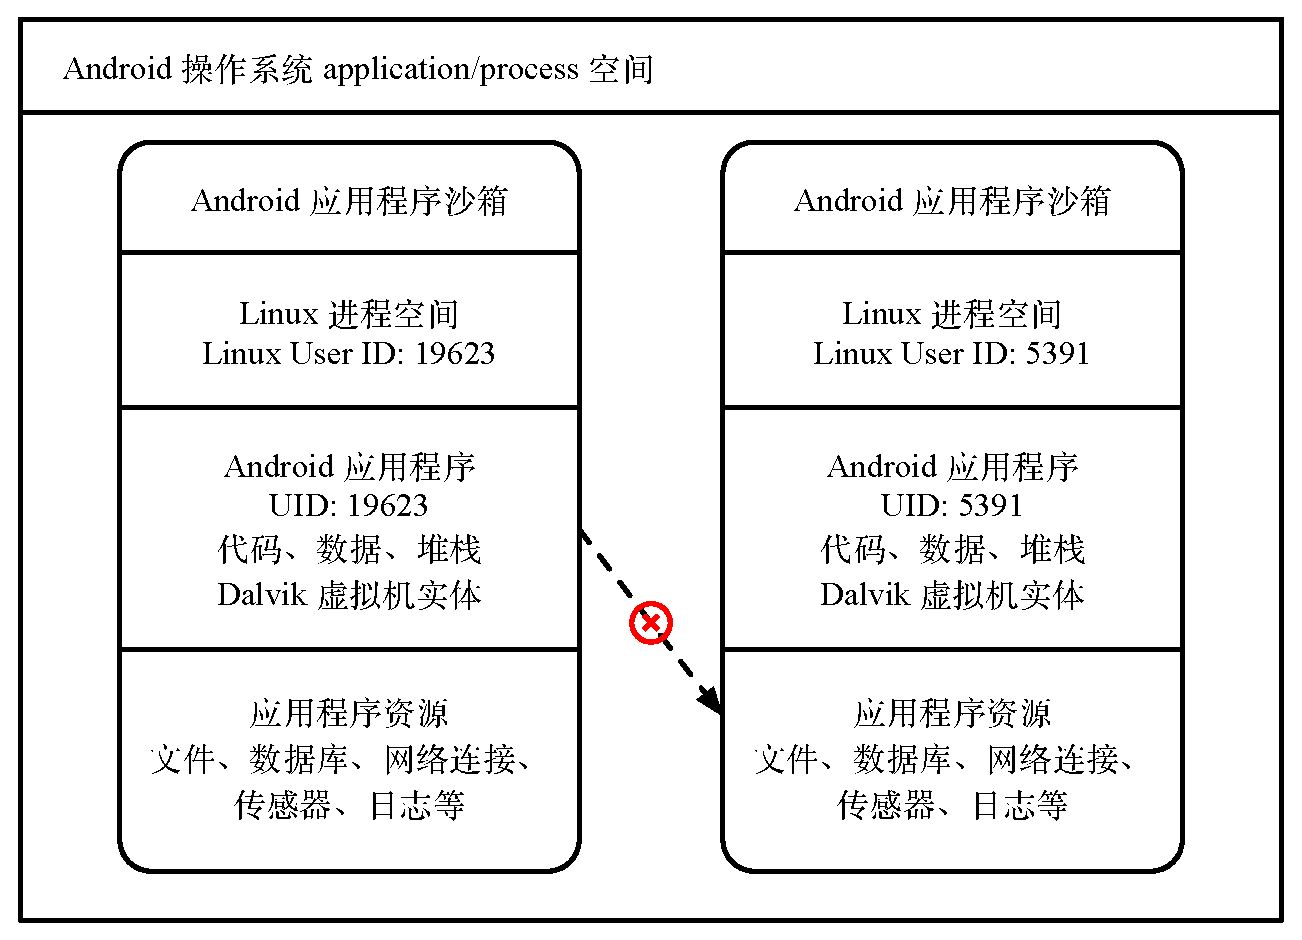
\includegraphics[width=.3\linewidth]{figures/content/2_1}
    \caption{错误的书脊渲染}
    \label{fig:2_1}
    \end{minipage}
    \begin{minipage}[t]{0.3\textwidth}
    \centering
    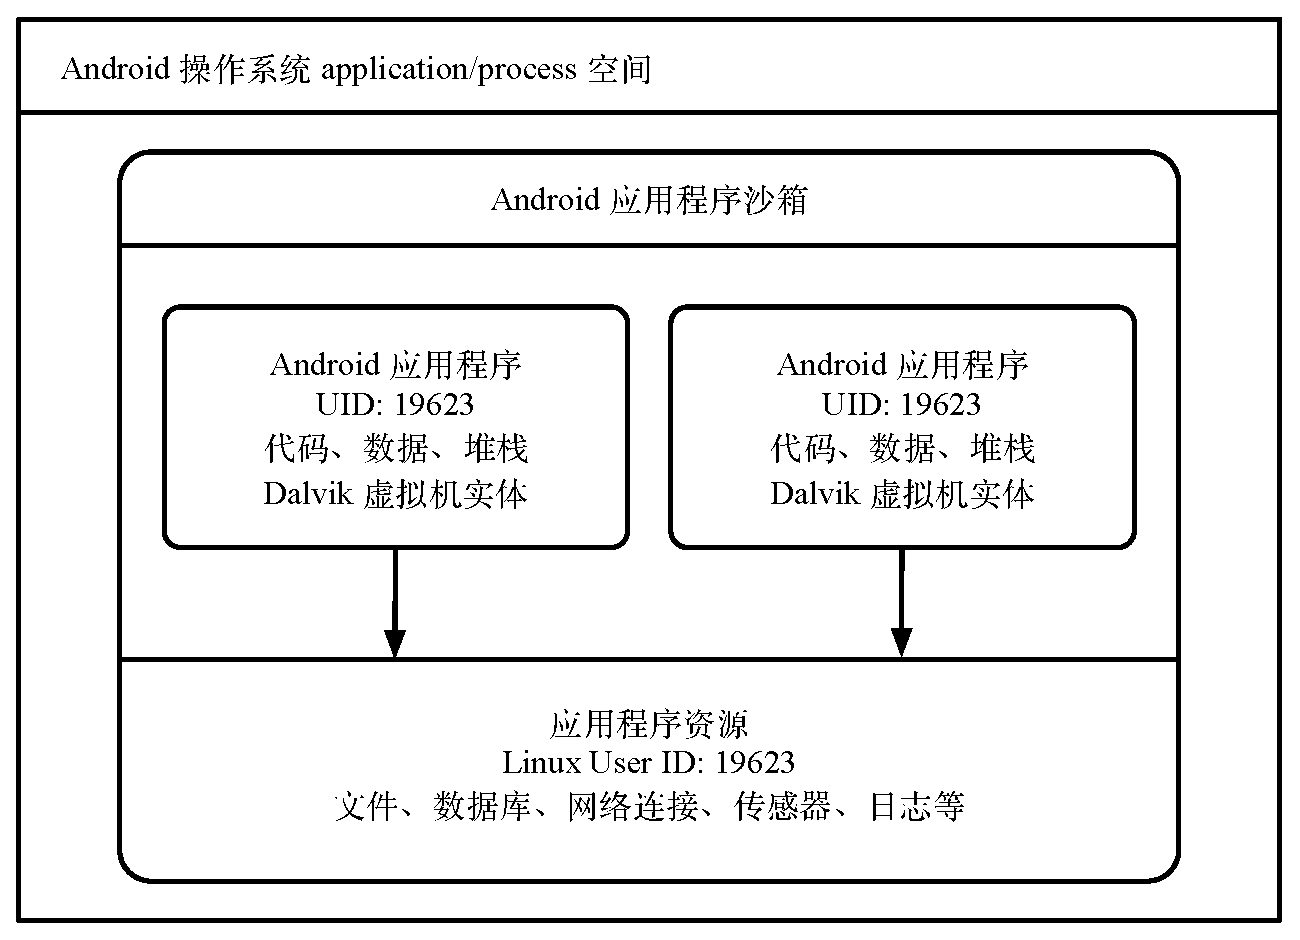
\includegraphics[width=.3\linewidth]{figures/content/2_2}
    \caption{西文旋转后的书脊渲染}
    \label{fig:2_2}
    \end{minipage}
    \begin{minipage}[t]{0.3\textwidth}
    \centering
    
\includegraphics[width=.3\linewidth]{figures/content/2_3}
    \caption{提升基线后的书脊渲染}
    \label{fig:2_3}
    \end{minipage}
\end{figure}

\noindent 这时你必须显式地指定书脊的渲染方式。指定的方式很简单,你只需告知编译引擎对标题中的西文字母进行逆时针270$^{\circ}$(即顺时针90$^{\circ}$)旋转即可:

\begin{tcolorbox}
\begin{lstlisting}[language=TeX]
\spine
    {面向种群的 \rotatebox{270}{Android} 安全风险评估和恶意应用检测}
    {}
\end{lstlisting}
\end{tcolorbox}

\noindent 请注意,{\codefont $\backslash$rotatebox\{270\}\{\}}前后应该各留一个空格,否则会导致编译错误。和论文标题类似,没有副标题时上述第2个字段可以留空。这样修正后的书脊渲染如图 \ref{fig:2_2} 所示。尽管如此,你仍然能从图 \ref{fig:2_2} 中注意到一些异常。拉丁字母在旋转之后的基线高度比汉字基线高度略低,因此导致书脊中的西文部分看起来总是偏左。解决这一问题,你可以在旋转命令中嵌套基线提升命令,就像这样:

\begin{tcolorbox}
\begin{lstlisting}[language=TeX]
\spine
  {面向种群的 \rotatebox{270}{\raisebox{2.5pt}{Android}} 安全风险评估和恶意应用检测}
  {}
\end{lstlisting}
\end{tcolorbox}

再次修正后的书脊渲染如图 \ref{fig:2_3} 所示,这时你就得到了完美的中西文混排书脊。再次强调,如果你的论文标题中没有中西文混排,请直接删去{\codefont $\backslash$spine}字段。

\section{作者与导师}

该部分用于指定论文的作者与导师姓名。作者字段分为2个部分,分别是作者的中文名及其拉丁文转写:

\begin{tcolorbox}
\begin{lstlisting}[language=TeX]
\author
    {陈仁营}
    {CHEN Ren-ying}
\end{lstlisting}
\end{tcolorbox}

\noindent 关于中文姓名转写为英文时的拼写规则,根据《东南大学研究生学位论文格式规定》\cite{seugs2015rule}第一条第二款之要求,有如下规定:

~

\noindent{\color{black!45}
中国姓名译为英文时用汉语拼音,按照姓前名后的原则,姓、名均用全名,不宜用缩写。姓全用大写,名的第一个字母大写,名为双中文字时两个字的拼音之间可以不用短划线,但容易引起歧义时必须用短划线。例如“冯长根”译为“FENG Changgen”或“FENG Chang-gen”,而“冯长安”则必须译为“FENG Chang-an”。论文英文封面上的署名也遵守此规定。}

~

导师字段分为3个部分,分别是导师的中文名、姓名的拉丁文转写以及导师的英文职称,用于显示在英文封面上:

\begin{tcolorbox}
\begin{lstlisting}[language=TeX]
\advisor
    {张广军}
    {ZHANG Guang-Jun}
    {Prof.}
\end{lstlisting}
\end{tcolorbox}

\noindent 对于硕士研究生和博士研究生,导师的职称一般为副教授级及以上。导师为副教授的,职称可以写全称 Associate Professor,也可以写简称 A. Prof.;导师为教授的,可以写全称 Professor或简称Prof.,注意上述简称中的~.不可省略。对于导师职称未达副教授级的特殊情况,比如导师职称为讲师时,请勿在职称处填写Lecturer,此时宜填写Doctor或Dr.以示尊重。

一些硕士研究生可能会有副导师,此时可以显式指定副导师的相关信息,具体方法和导师相同:

\begin{tcolorbox}
\begin{lstlisting}[language=TeX]
\coadvisor
    {程光}
    {CHENG Guang}
    {Prof.}
\end{lstlisting}
\end{tcolorbox}

\noindent 没有副导师的研究生学位论文,请删去上述几行。

\section{答辩信息}

答辩信息用于在论文A3封面和中文彩色封面中渲染与研究生论文答辩相关的信息。

\begin{tcolorbox}
\begin{lstlisting}[language=TeX]
\degreetype{工学硕士}{Master of Engineering}
\major{生物医学工程}
\submajor{神经信息工程}
\defenddate{2020年1月20日}
\authorizedate{2020年1月23日}
\committeechair{齐康}
\reviewer{王建国}{韩冬青}
\department{网络空间安全学院}{School of Cyberspace Security}
\seuthesisthanks{本文的部分工作受国家自然基金 No. wdnmd666 的支持与帮助,在此表示感谢。}
\end{lstlisting}
\end{tcolorbox}

其中,{\codefont degreetype}字段用于指定所申请的学位类型与等级。{\codefont major}和{\codefont submajor}字段用于指定研究生攻读的一级和二级学科名称,请依照中华人民共和国教育部一级和二级学科名录进行填写。如果所属专业直接隶属于一级学科,{\codefont submajor}字段可以留空不填。{\codefont defenddate}和{\codefont authorizedate}分别用于指定论文的答辩日期和学位的授予日期,请根据实际情况填写。{\codefont committeechair}和{\codefont reviewer}用于指定论文的答辩委员会主席和论文评阅人。根据《东南大学研究生学位论文格式规定》\cite{seugs2015rule}第二条第一款之要求,有如下规定:

~

\noindent{\color{black!45}
论文印刷时尚无法填写的评阅人和答辩委员会主席等栏目待答辩完成后要填写补齐,不要空缺。盲审论文的评阅人处标明“盲审”。}

~

{\codefont department}字段用于指定研究生所属的院系,其中院系的英文名将用于英文封面的生成。学院的正确英文译名请查阅所属学院的官方网站。{\codefont seuthesisthanks}用于在论文的中文内页页脚处对论文所属的项目、赞助的基金课题进行简短的鸣谢。此处不宜书写大段文字,请用简单的一两句话对相关组织或机构表示感谢,对其他个人的感谢请在文尾的致谢部分进行。没有相关赞助的学位论文请直接删去该字段。

\section{模板参数}

你有可能已经注意到了在main.tex文件中引入模板类的命令里包含了若干模板参数:

\begin{tcolorbox}
\begin{lstlisting}[language=TeX]
\documentclass[algorithmlist,figurelist,tablelist,nomlist]{seumasterthesis}
\end{lstlisting}
\end{tcolorbox}

\noindent 即{\codefont documentclass}命令后的中括号里的几个参数。这些参数用于控制条件编译以及在论文渲染时向模板类提供额外的信息。本节将会介绍本模板提供的模板参数及其具体含义。

\subsection{链接着色}

本模板通过使用hyperref宏包来提供索引和链接跳转功能。相信你已经注意到了,本模板所渲染出的PDF文档中的所有图片、表格、公式、算法和参考文献索引都被着色高亮,且可以通过点击跳转到原引位置。该功能便于读者在阅读电子文档时快速定位相应索引的位置,但是着色高亮的链接在论文付梓时可能会影响到印刷效果。因此,本模板提供了针对链接着色的模板参数。通过在模板参数列表中添加{\codefont nocolorlinks}参数,模板所渲染出的PDF文档中的所有文献索引都将被取消着色,以便论文的正式印刷。

\subsection{图表、算法及术语目录}

根据不同院系和专业的具体情况,硕士研究生学位论文可能并不需要图表、算法或术语目录中的一项或多项。尽管本模板默认会渲染出上述的所有目录,但是我们也提供了相应的模板参数来灵活控制这些目录的渲染。如果你在模板参数列表中显式指定{\codefont figurelist},代表你希望在论文编译时在章节目录后添加图片目录;类似的,{\codefont tablelist}显式指定了表格目录的需求,{\codefont nomlist}指定了术语表,而{\codefont algorithmlist}指定了算法目录。需要注意的是,你并不需要关注这几个模板参数在参数表中的位置或顺序,具体目录的编译和渲染仍然会依照《东南大学研究生学位论文格式规定》\cite{seugs2015rule}第一条中所规定的顺序进行。

\subsection{硕士类型}

本模板同时支持学术型硕士研究生和专业型硕士研究生。当不添加任何模板参数时,该模板将默认渲染为学术型硕士研究生学位论文;而当在模板参数列表中显式指定{\codefont engineer}时,该模板将渲染为专业型硕士研究生学位论文。两种论文的主要区别在于 A3 大封面和中文彩色封面的标题,学术型硕士研究生为《硕士学位论文》,而专业型硕士研究生一般为《工程硕士学位论文》。需要注意的是,中文内页封面的标题在两种类型的硕士研究生学位论文中都为《硕士学位论文》。此外,若干年之前的一些专业型硕士学位论文的偶数页页眉为“东南大学工程硕士学位论文”,但近几年的论文中未发现这种区别,《东南大学研究生学位论文格式规定》中也未对此有相关规定,因此我们没有进行多余的设置。
\chapter{系统框架设计}

	本节介绍AppWrapper工具包。与传统的appwrapping技术不同,此工具包可以在字节码级别添加安全功能,以使方法单元上的应用程序不安全,并控制是否通过动态策略管理启用安全功能。如图\ref{fig_1}所示,AppWrapper工具包由三部分组成:自动app包装,实时app流确认和策略设置,以及动态策略管理。
	
	\begin{figure}[hbt]
		\centering
		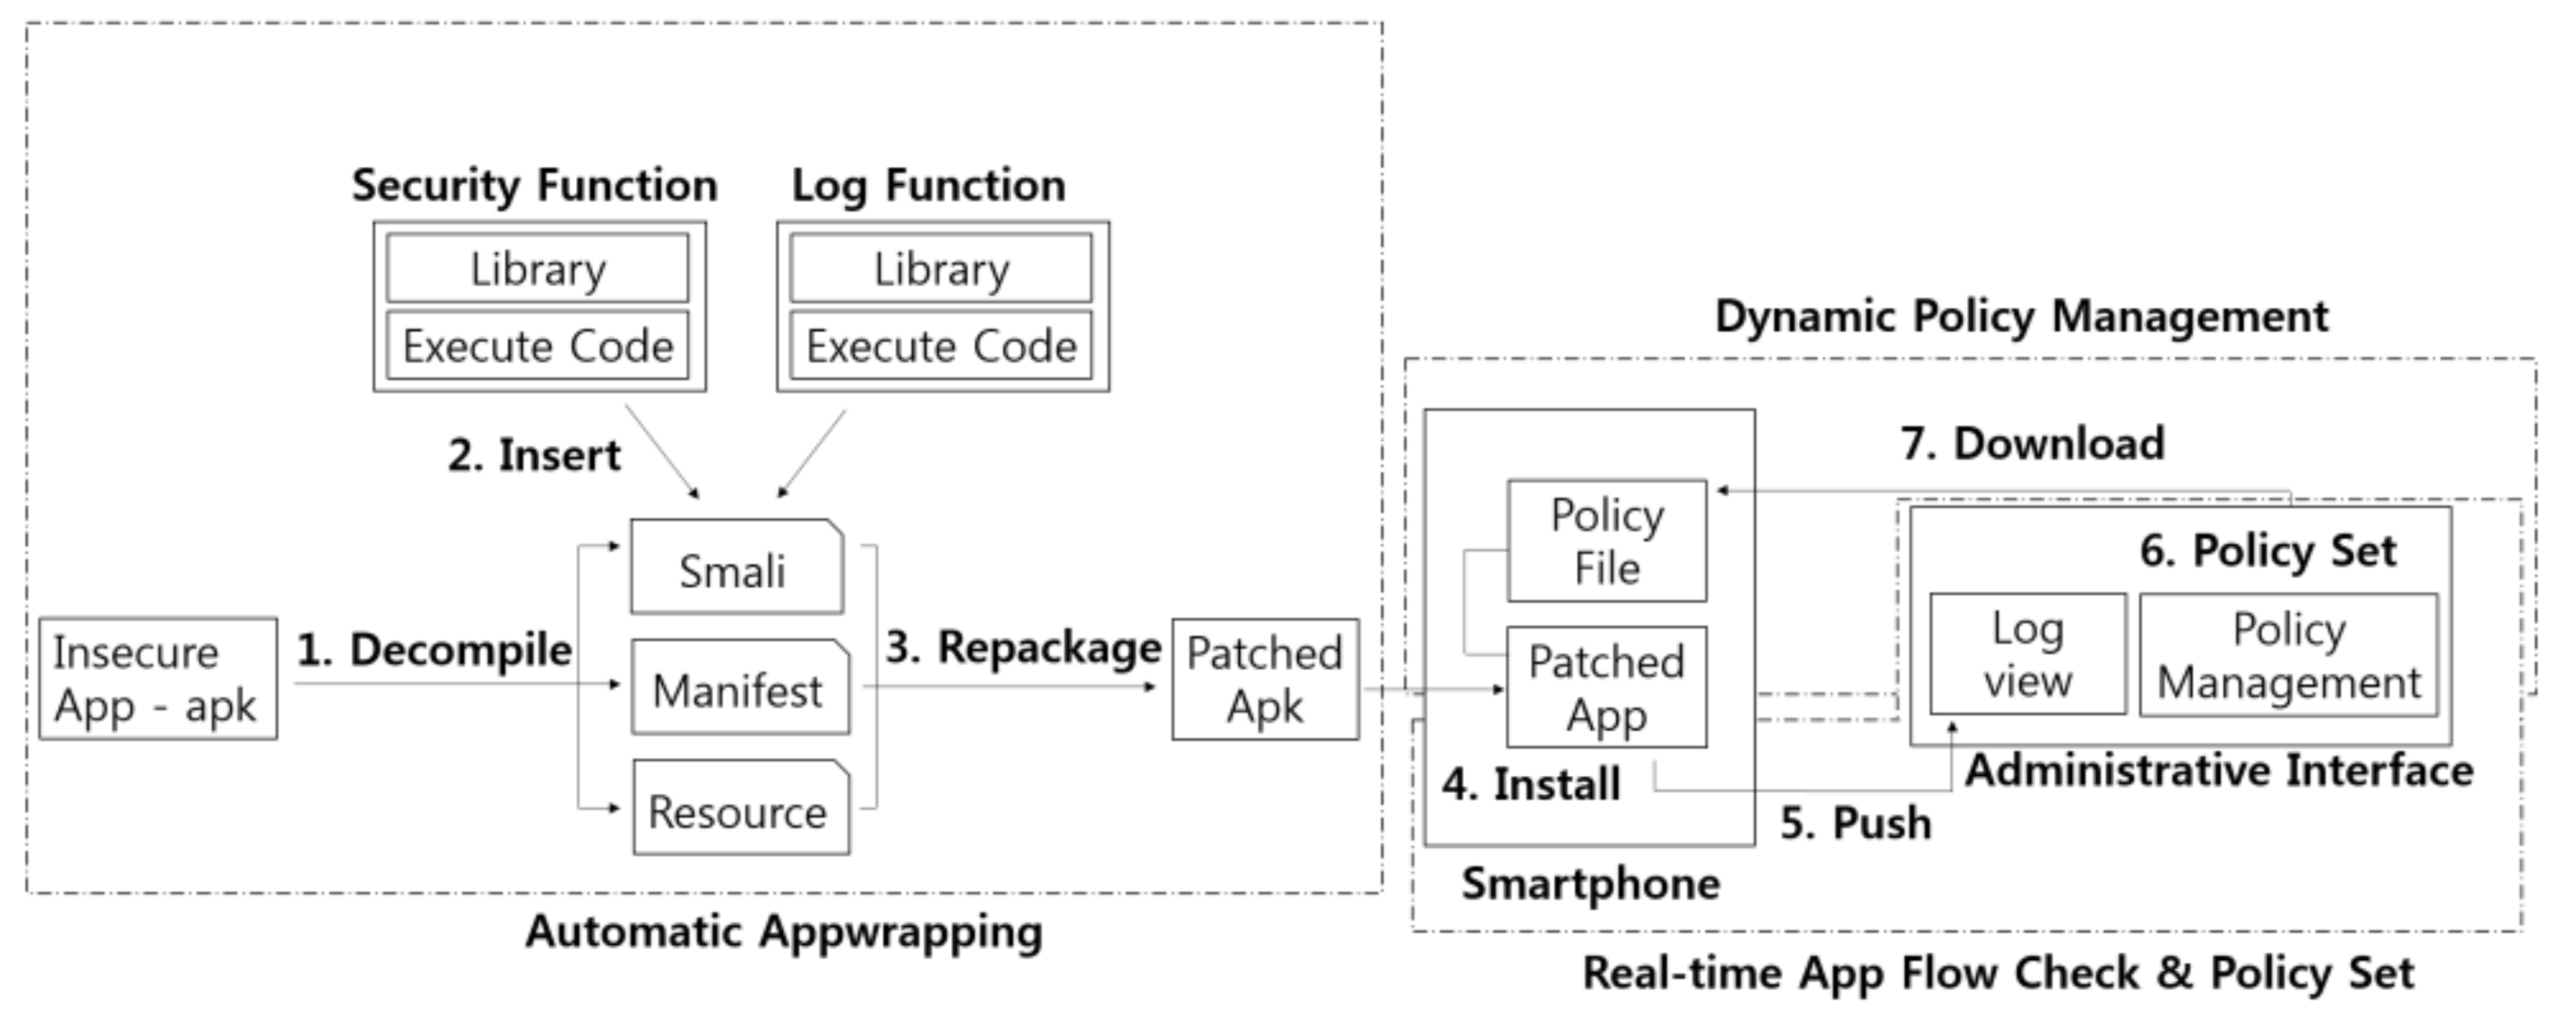
\includegraphics[width=.7\textwidth]{fig1}
		\caption{AppWrapper 概述}
		\label{fig_1}
	\end{figure}

	
	\begin{enumerate}
		\item 反编译不安全应用程序的.apk以获取smali文件作为字节码级别,AndroidManifest.xml文件和资源文件。
		\item 在步骤1中添加在smali code和smali文件中提取的安全性功能和日志应用程序功能。
		\item 使用安全功能和日志功能,现有AndroidManifest.xml文件和资源文件重新打包smali文件,以创建修补的.apk文件。
		\item 在智能手机上安装生成的.apk文件。
		\item 运行已修补的应用程序时,驱动信息(活动类名称,方法名称)将根据应用程序进度的流程发送到AppWrapper工具箱的UI的日志视图。
		\item 检查日志视图并根据应用程序的进度流程将策略设置为在需要安全功能的位置运行安全功能。
		\item 一旦设置了所有必要的安全策略,请将策略文件下载到用户的电话并运行修补的应用程序。修补应用程序的安全功能根据应用程序的进度与下载的策略文件一起执行。
	\end{enumerate}

	该流程在以下小节中详细描述。

	\section{应用程序自动包装}
		安全和日志记录功能是在字节码级别添加的,没有Android的原始源代码。有必要对不安全应用程序的.apk文件进行反编译和重新打包(重新编译和签名)。使用apktool.jar文件执行反编译和重新编译过程。通过重新编译获得的.apk文件使用signapk.jar文件进行签名,并转换为可以安装在用户手机中的.apk文件。签名时需要签名密钥。

		通过反编译.apk获得的smali文件是在字节码级别用smali编写的代码集合,其中添加了安全功能和日志功能。添加的位置是活动中的所有方法单位。它被添加到AndroidManifest.xml文件中声明的所有活动类中的所有方法中。安全和日志函数的smali代码被添加到每个方法的开头,以最小化与现有代码的冲突。在smali中,.method和end方法语法分别表示方法的开始和结束。

		在smali中,寄存器区域根据每个方法中声明的局部变量和输入参数的数量进行分配。在要分配的寄存器区域中有4位,8位和16位,并且对于这些分配中的每一个,指令是不同的。安全性和日志功能代码使用三个局部变量。对于4位寄存器,可以使用从0到15的16个地址编号.Ifa16th addressisusedina4bit寄存器分配方法,发生寄存器错误,重新编译过程失败。为了避免这个问题,通过计算方法中局部变量和参数的数量,将安全性和日志函数添加到仅13个或更少的局部变量分配方法中。这允许添加安全性和日志功能,然后重新打包而不会出现错误。

	\section{动态策略执行}
	
		\begin{figure}[hbt]
			\centering
			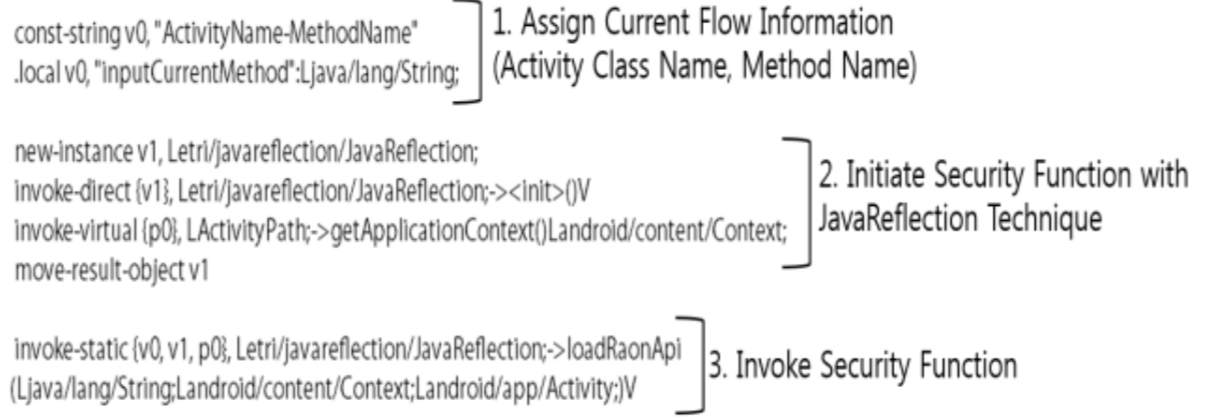
\includegraphics[width=.7\textwidth]{fig2}
			\caption{使用java反射的Smali安全功能代码}
			\label{fig_2}
		\end{figure}

		通过appwrapping添加的安全功能由策略决定。现有的应用程序技术在动态策略管理中存在困难,因为所有与安全相关的代码都包含在基于静态策略添加的安全功能中。但是,建议的AppWrapper可以使用Java反射技术基于动态策略调用和管理各种安全功能。 Java反射技术是一种用于动态加载和使用类的流行技术。通过应用这种技术调用安全函数的smali代码如图\ref{fig_2}所示。当调用安全函数时,它被指定为变量,以便它可以作为参数传输到哪个位置(类名和方法名)叫做。然后,使用Java反射技术初始化安全性函数库,并且与先前分配的变量(类名和方法名)一起调用安全性函数。通过该流程,可以根据app的进度在方法单元中执行安全功能,并且可以灵活地应用各种安全功能。另外,在添加第一个安全功能之后,不需要再次添加安全功能和重新打包过程。由于已将所有安全功能添加到所有方法单元,因此当将新创建的具有已更改策略的策略文件下载到用户的电话时,将自动应用新策略。
				
		可以通过管理界面执行策略设置和管理,如图\ref{fig_3}所示。管理界面由三个单独的屏幕组成:活动类列表和所选活动类和安全功能列表的方法列表。要设置策略,请选择要添加安全功能的活动类,然后选择在活动中执行安全功能的方法位置。然后选择要执行的安全功能。策略设置完成后,将创建策略文件。策略文件包括要执行的安全功能库信息和安全功能信息,以及执行安全功能的位置信息(活动类,方法名称)。表\ref{tab1}显示了一个示例策略文件。安全功能库信息用于使用上述Java反射技术动态调用安全功能。
		
		\begin{table}
			\centering
			\caption{策略文件样本}
			\label{tab1}
			\begin{tabular}{|c|c|c|c|c|}
				\hline
				\# & 活动类 & 方法名 & 安全库 & 安全函数\\
				\hline
				1 & MainActivity & onResume & SecurityApi, SecurityFuntion & FIDO Authentication\\
				\hline
				2 & LoginActivity & onCreate & SecurityApi, SecurityFuntion & Office Model Login\\
				\hline
				3 & LoginActivity & onResume & SecurityApi, SecurityFuntion & Office Model Logout\\
				\hline
			\end{tabular}
		\end{table}

	\section{检查实时应用程序行为并设置策略}
	
		将安全功能添加到不安全的应用程序时,将检查应用程序的进度。 为此,添加了一个日志功能以查看实时应用程序行为。 日志功能使用SSL连接到AppWrapper工具包,并根据应用程序进度流传输日志信息。 通过appwrapping将日志功能添加到修补的应用程序中。 启动修补应用程序后,您可以根据应用程序的流程检查日志信息(类名,方法名称),如图\ref{fig_4}所示。如果单击要设置策略的位置的日志, 您将切换到图\ref{fig_5}的策略设置用户界面屏幕。如果设置策略,则根据应用程序进度流程将安全功能添加到缺乏安全性的位置。
		
		\begin{figure}[hbt]
			\centering
			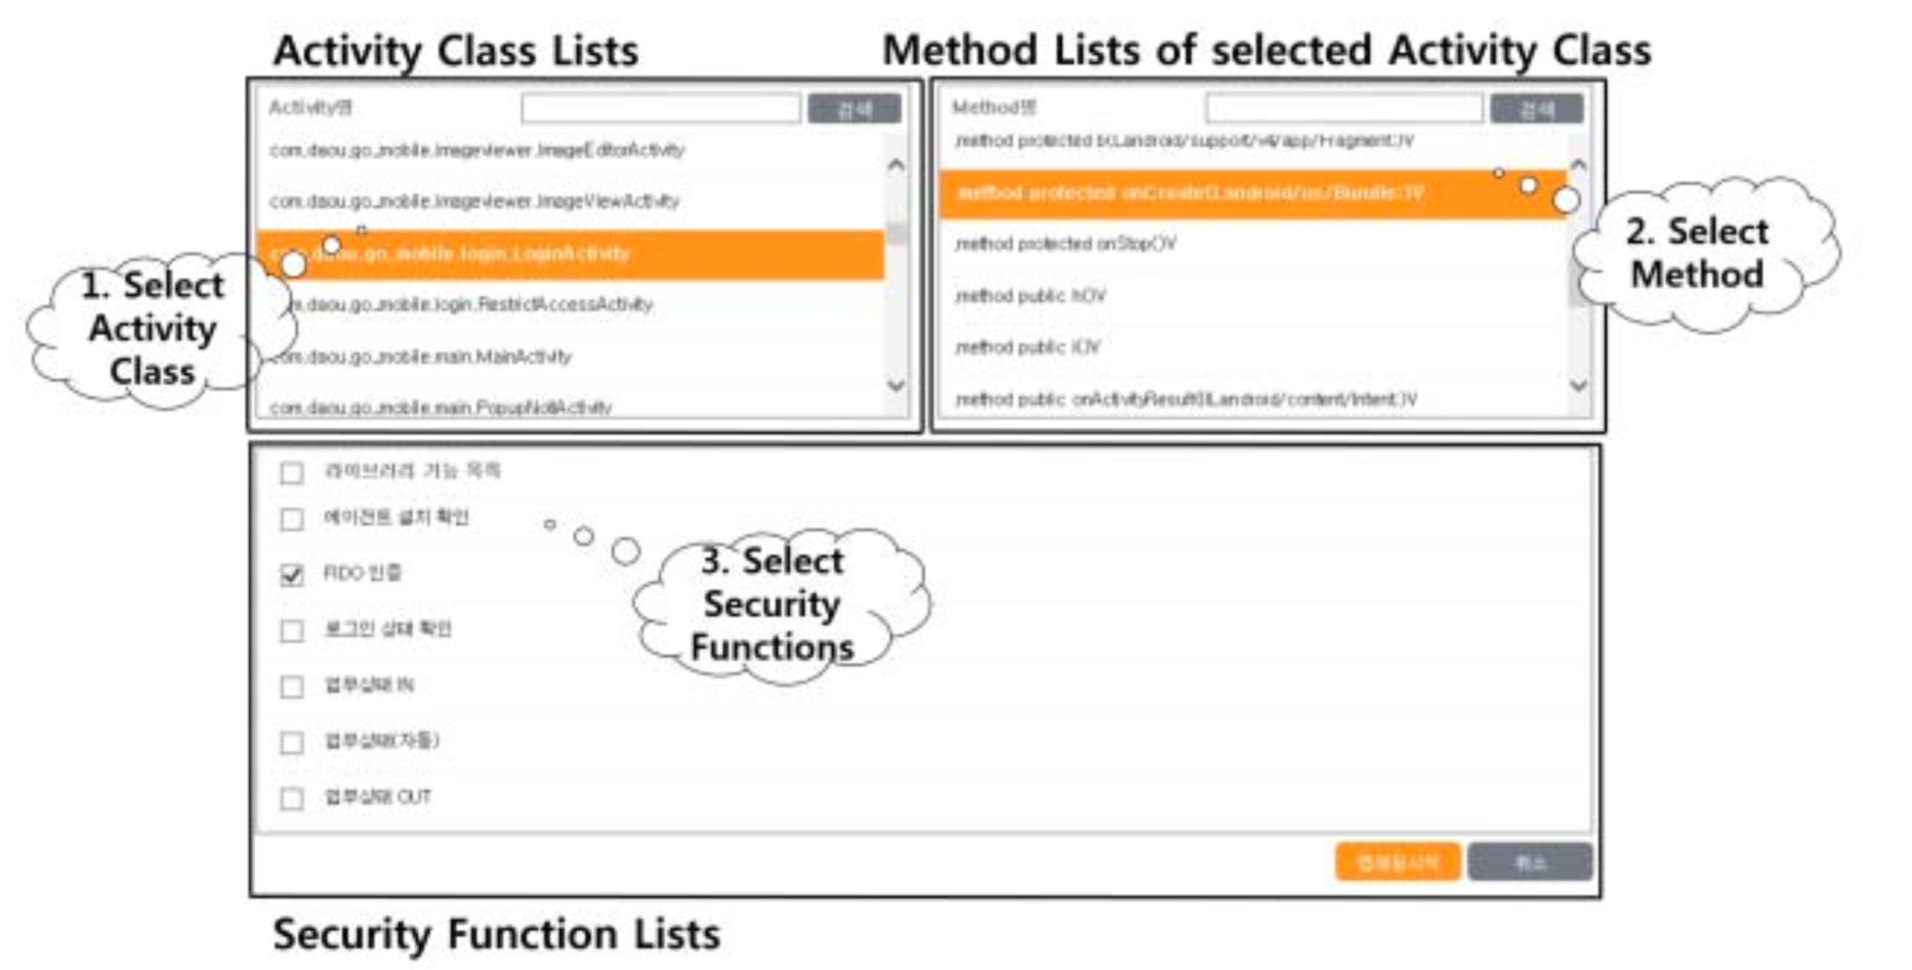
\includegraphics[width=.7\textwidth]{fig3}
			\caption{动态策略管理界面}
			\label{fig_3}
		\end{figure}
		
		\begin{figure}[hbt]
			\centering
			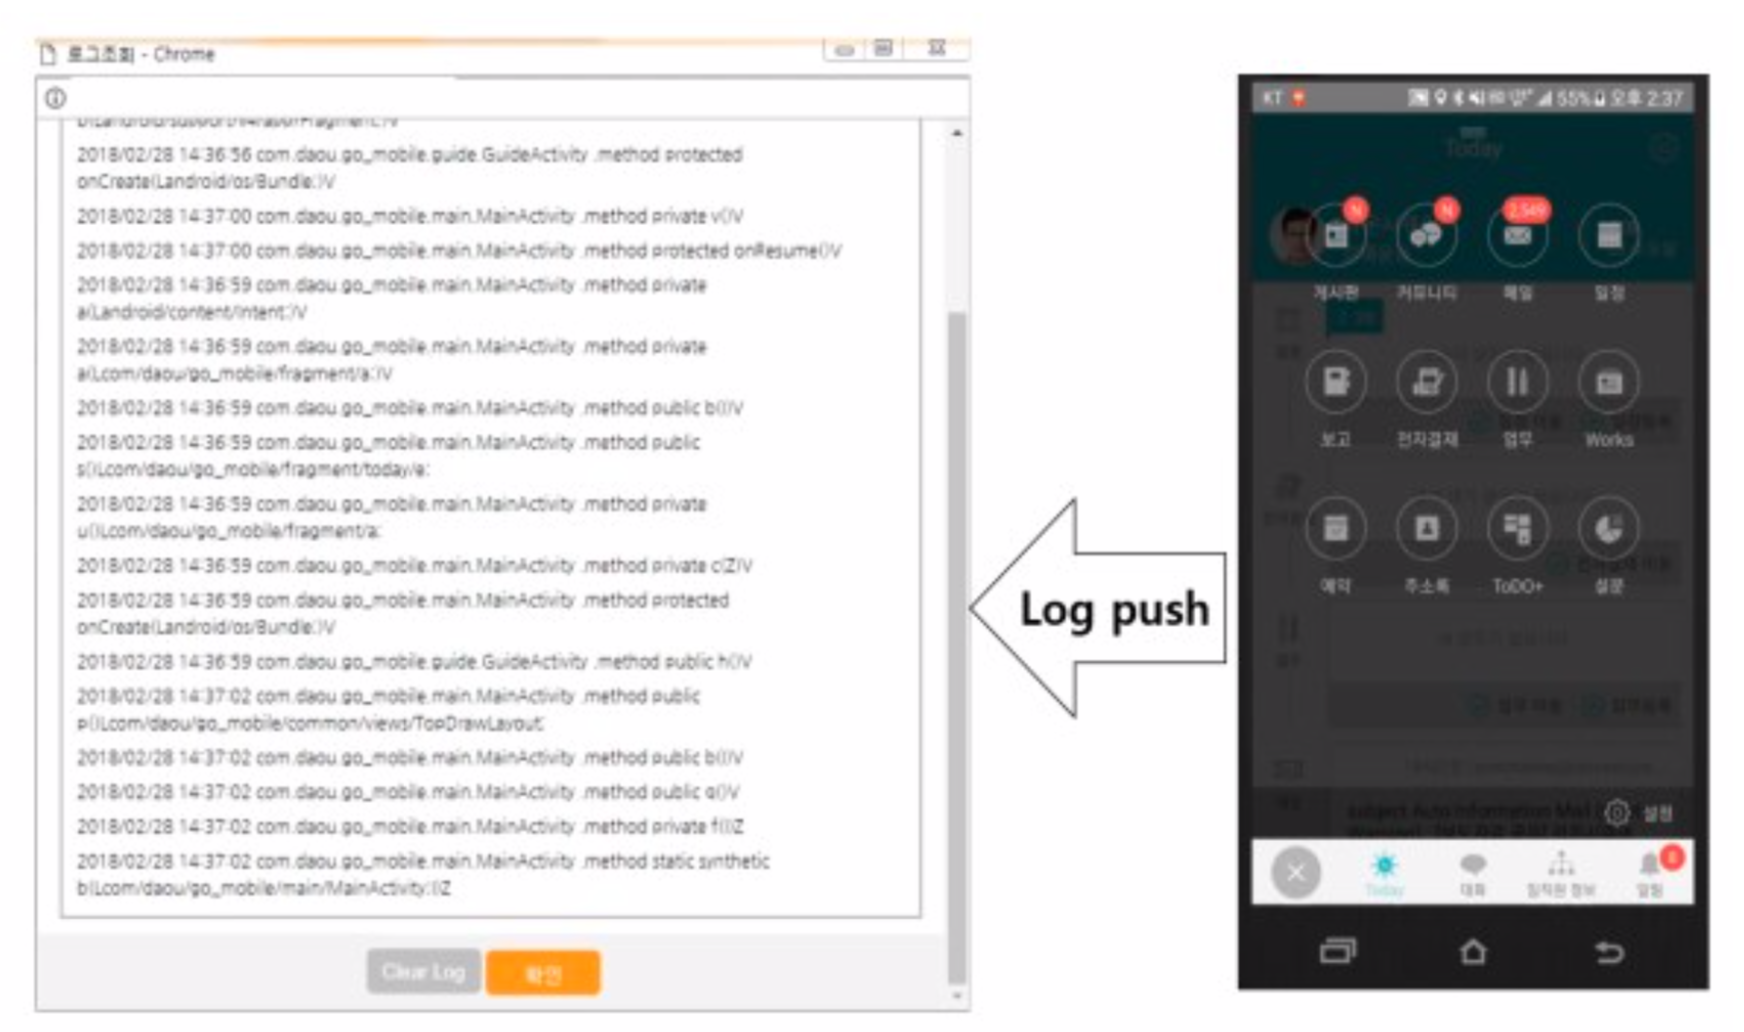
\includegraphics[width=.7\textwidth]{fig4}
			\caption{实时日志视图管理界面}
			\label{fig_4}
		\end{figure}
		
		\begin{figure}[hbt]
			\centering
			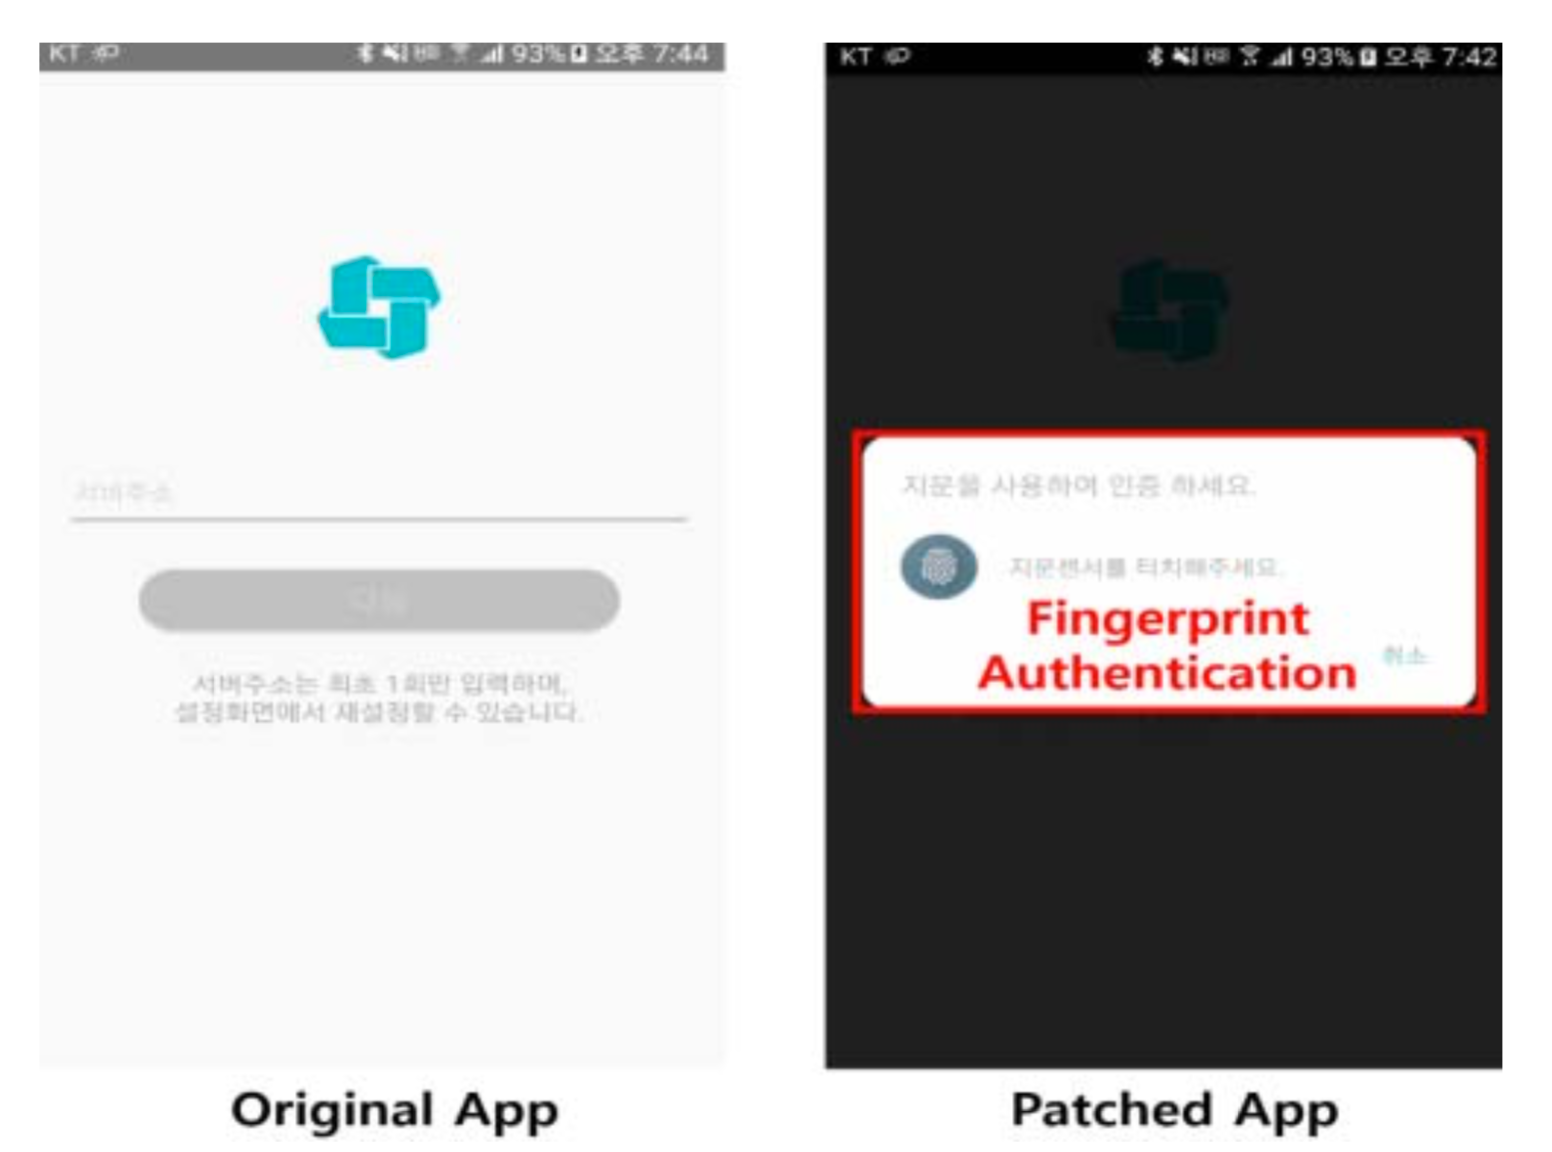
\includegraphics[width=.7\textwidth]{fig5}
			\caption{安全功能补丁前/后的应用启动屏幕}
			\label{fig_5}
		\end{figure}
\chapter{特殊环境与浮动体}
\label{chp:float}

事实上我们本该假设所有使用本 \LaTeX 论文模板的人都具备了相当的 \LaTeX 使用经验和知识,如果这样那么本章所介绍的内容是不言自明的。但是也存在很多初次接触 \LaTeX 的研究生朋友,因为各种不同的原因而尝试使用 \LaTeX 进行论文排版。因此我们认为还是有必要对这些 \LaTeX 中的基本元素进行反复地强调,以避免我们的个别开发者的邮箱和GitHub Issues被投诉和问询填满。如果你是一个 \LaTeX 老手,你可以直接跳过本章而不用担心漏过任何重要内容。

\section{图片}

\subsection{插入图片}
在 \LaTeX 文档中插入图片,你需要如下的代码:

\begin{tcolorbox}
\begin{lstlisting}[language=TeX]
\begin{figure}[htbp]
  \centering
  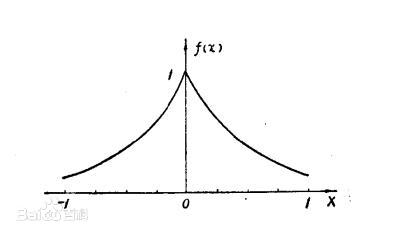
\includegraphics[width=.5\linewidth]{figures/content/4_1}
  \caption{插入图片示例}
  \label{fig:4_1}
\end{figure}
\end{lstlisting}
\end{tcolorbox}

\noindent 上面的代码会插入如下效果的图片:

\begin{figure}[htbp]
  \centering
  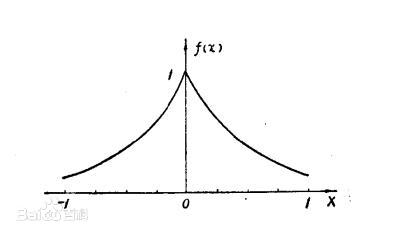
\includegraphics[width=.3\linewidth]{figures/content/4_1}
  \caption{插入图片示例}
  \label{fig:4_1}
\end{figure}

\subsection{浮动体环境与位置标识符}

\begin{tcolorbox}
\begin{lstlisting}[language=TeX]
\begin{figure}[htbp]
\end{figure}
\end{lstlisting}
\end{tcolorbox}

\noindent 声明了一个图片浮动体环境。浮动体是 \LaTeX 中的一种特殊容器,用于容纳占据篇幅较大但不方便分页的内容,如图片或表格。方括号中的字母是浮动体位置标识符,用于向 \LaTeX 编译引擎提出位置建议。常见的位置标识符有以下4种:

\begin{itemize}
  \item {\codefont h}:表示here。\LaTeX 编译引擎在面对用{\codefont h}标识的浮动体时会首先尝试在声明位置插入浮动体;
  \item {\codefont t}:表示top。\LaTeX 编译引擎会尝试在当页顶部安置浮动体;
  \item {\codefont b}:表示bottom。\LaTeX 编译引擎会尝试在当页底部安置浮动体;
  \item {\codefont p}:表示float page。\LaTeX 编译引擎会尝试为该浮动体分页并使其占据全页。
\end{itemize}
你可以使用多个位置标识符并将其自由组合,你指定的顺序代表你向 \LaTeX 编译引擎所推荐的优先级。需要说明的是,编译引擎并不保证会按照你所指定的位置优先级安置浮动体,而是会根据浮动体大小、其在页面中的位置、文字的相对分布等多种因素决定浮动体的位置。因此在论文写作过程中,我们不建议你使用如“下图”,“上表”等使用方位来指代特定图片或表格的表述,因为你所插入的图片或表格很有可能并不会被编译到你想要它出现的位置。当然,你也可以在标识符前加上 !号来表示强制位置,如{\codefont !h}。但是我们不推荐这样做,因为这可能会造成很多你意想不到的后果。

\subsection{图片的大小与路径}

\begin{tcolorbox}
\begin{lstlisting}[language=TeX]
\centering
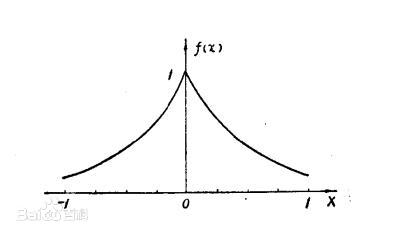
\includegraphics[width=.5\linewidth]{figures/content/4_1}
\end{lstlisting}
\end{tcolorbox}

{\codefont centering}表示浮动体在控制范围内居中。{\codefont includegraphics}语句向编译引擎指定你所想要引入的图片的大小与保存路径。在该命令之后跟随的方括号中,你可以指定图片的长或宽。默认情况下 \LaTeX 会锁定图片的长宽比例,因此你只需要指定长宽中的一个即可。后面的大括号用于填写图片的路径,你可以使用主文件main.tex的相对路径来表示。我们在模板根目录下设置了一个名为figures的目录用于存放图片,我们建议你把论文需要的所有图片放置于该目录下的content文件夹中以便查找和管理。

\subsection{图片的标题与标签}

\begin{tcolorbox}
\begin{lstlisting}[language=TeX]
\caption{插入图片示例}
\label{fig:4_1}
\end{lstlisting}
\end{tcolorbox}

{\codefont caption}用于指定图片的标题。{\codefont label}用于给图片添加标签,便于你在文本中引用该图片。对于上面的图片,如果我们想要在论文中引述其内容,可以采用如下方法:

\begin{tcolorbox}
\begin{lstlisting}[language=TeX]
图\ref{fig:4_1}是东南大学的校徽,它的设计中蕴含着多种寓意。
\end{lstlisting}
\end{tcolorbox}

\noindent 上述文本在编译后会呈现这样的效果:

图\ref{fig:4_1}是东南大学的校徽,它的设计中蕴含着多种寓意。

\subsection{图片的并排}

很多时候,你可能会想要将两张图片并排放置以节省排版空间。我们支持并鼓励你这样做。你只需要引入如下的代码:

\begin{tcolorbox}
\begin{lstlisting}[language=TeX]
\begin{figure}[htbp]
  \centering
    \begin{minipage}[t]{0.48\textwidth}
      \centering
      
\includegraphics[width=6cm]{figures/content/4_2}
      \caption{GitHub}
      \label{fig:4_2}
    \end{minipage}
    \begin{minipage}[t]{0.48\textwidth}
      \centering
      
\includegraphics[width=8cm]{figures/content/4_3}
      \caption{NPM}
      \label{fig:4_3}
    \end{minipage}
\end{figure}
\end{lstlisting}
\end{tcolorbox}

\noindent 编译后的效果是这样的:

\begin{figure}[htbp]
  \centering
    \begin{minipage}[t]{0.48\textwidth}
      \centering
      
\includegraphics[width=4cm]{figures/content/4_2}
      \caption{GitHub}
      \label{fig:4_2}
    \end{minipage}
    \begin{minipage}[t]{0.48\textwidth}
      \centering
      
\includegraphics[width=3cm]{figures/content/4_3}
      \caption{npm}
      \label{fig:4_3}
    \end{minipage}
\end{figure}

注意,在上述代码中,我们定义了一个{\codefont figure}浮动体环境,并在其中用两个:

\begin{tcolorbox}
\begin{lstlisting}[language=TeX]
\begin{minipage}[t]{0.48\textwidth}
\end{minipage}
\end{lstlisting}
\end{tcolorbox}

\noindent 包裹了两张图片的声明。和单个图片类似,你也可以指定{\codefont minipage}相对浮动体的位置和大小。编译引擎将根据你{\codefont minipage}的大小调整在一行显示的图片数量。需要注意的是,在两个{\codefont minipage}声明之间请勿空行,因为 \LaTeX 编译引擎会将空行视作换行请求而错误地将你的两张图片上下放置。

\section{表格}

\subsection{插入表格}

在论文中插入表格的方法与图片类似,示例代码如下:

\begin{tcolorbox}
\begin{lstlisting}[language=TeX]
\begin{table}[htbp]
\centering
\caption{东南大学院系表}
\label{tab:4_1}
\begin{tabular}{cll}
\toprule
院系编号&\multicolumn{1}{c}{院系名称}&\multicolumn{1}{c}{院系英文译名}\\
\midrule
01  & 建筑学院      & School of Architecture  \\
02  & 机械工程学院    & School of Mechanical Engineering \\
03  & 能源与环境学院   & School of Energy and Environment \\
04  & 信息科学与工程学院 & School of Information Science and Engineering \\
05  & 土木工程学院    & School of Civil Engineering \\
\bottomrule
\end{tabular}
\end{table}
\end{lstlisting}
\end{tcolorbox}

\noindent 编译后的效果如表 \ref{tab:4_1} 所示。想要定义一个表格,首先需要声明浮动体环境:

\begin{table}[htbp]
\centering
\caption{东南大学院系表}
\label{tab:4_1}
\begin{tabular}{cll}
\toprule
院系编号 & \multicolumn{1}{c}{院系名称}       & \multicolumn{1}{c}{院系英文译名 }     \\
\midrule
01                       & 建筑学院      & School of Architecture                        \\
02                       & 机械工程学院    & School of Mechanical Engineering              \\
03                       & 能源与环境学院   & School of Energy and Environment              \\
04                       & 信息科学与工程学院 & School of Information Science and Engineering \\
05                       & 土木工程学院    & School of Civil Engineering \\
\bottomrule
\end{tabular}
\end{table}

\begin{tcolorbox}
\begin{lstlisting}[language=TeX]
\begin{table}[htbp]
  \centering
  \caption{东南大学院系表}
  \label{tab:4_1}
\end{table}
\end{lstlisting}
\end{tcolorbox}

\noindent 在声明表格浮动体时,你也可以指定该表格的标题和标签,这与图片的声明类似。需要提醒的是,根据《东南大学研究生学位论文格式规定》\cite{seugs2015rule}第一条第五款第六则的要求,表格的标题应该位于表格的上方,而图片的标题应该出现在图片的下方。

表格的具体内容在需要在浮动体中用{\codefont tabular}环境声明:

\begin{tcolorbox}
\begin{lstlisting}[language=TeX]
\begin{tabular}{cll}
  \toprule
  院系编号&\multicolumn{1}{c}{院系名称}&\multicolumn{1}{c}{院系英文译名}\\
  \midrule
  01  & 建筑学院      & School of Architecture  \\
  02  & 机械工程学院    & School of Mechanical Engineering \\
  03  & 能源与环境学院   & School of Energy and Environment \\
  04  & 信息科学与工程学院 & School of Information Science and Engineering \\
  05  & 土木工程学院    & School of Civil Engineering \\
  \bottomrule
\end{tabular}
\end{lstlisting}
\end{tcolorbox}

\noindent {\codefont tabular}声明后面紧跟着的是表格的纵向对其标准,比如我们的表格有3列,就需要使用3个字母分别指定这3列的对齐准则。你可以使用{\codefont l}表示左对齐,使用{\codefont r}表示右对齐,而使用{\codefont c}表示居中。下面你就可以以行为单位添加表格的内容,行与行间用两条反斜杠隔开,而行中的不同列间使用符号\&隔开。

需要特别注意的是,学术论文一般要求所有表格采用三线表形式。对于三线表,其列间不允许存在竖分割线,而行间仅在表顶、表头与表身、表尾处用三条横线确定表格的结构。因此在表格绘制时,你需要手动指定三线的位置,并在相应的行间添加下面三条指令,分别指代顶线、中间线和尾线:

\begin{tcolorbox}
\begin{lstlisting}[language=TeX]
\toprule
\midrule
\bottomrule
\end{lstlisting}
\end{tcolorbox}

~

事实上,在 \LaTeX 文本中插入表格确实需要付出很大的精力对表格的内容和样式进行调整,这也是很多初学者诟病 \LaTeX 的原因之一。为了方便你设计表格,我们向你推荐\href{http://www.tablesgenerator.com/}{一个网站},该网站能够使用图形化界面创建表格,然后自动生成对应的 \LaTeX 代码。你只需要把代码复制到你的文档中,并稍加调整与修正即可。

\section{算法}

一些理学和工学专业的研究可能需要在论文中插入为代码或算法,本模板同样支持这一功能。示例代码如下:

\begin{tcolorbox}
\begin{lstlisting}[language=TeX]
\begin{algorithm}
\caption{辗转相除法}
\label{alg:4_1}
\begin{algorithmic}
\Require 一个整数$m$
\Require 另一个整数$n$
\Ensure $m$和$n$的最大公约数$r$
\While {$n > 0$}
    \State $t \leftarrow m ~ mod ~ n$
    \State $m \leftarrow n$
    \State $n \leftarrow t$
\EndWhile
\State $r \leftarrow t$
\end{algorithmic}
\end{algorithm}
\end{lstlisting}
\end{tcolorbox}

\noindent 上述代码的编译结果如算法 \ref{alg:4_1} 所示。

\begin{algorithm}
\caption{辗转相除法}
\label{alg:4_1}
\begin{algorithmic}
\Require 一个整数$m$
\Require 另一个整数$n$
\Ensure $m$和$n$的最大公约数$r$
\While {$n > 0$}
    \State $t \leftarrow m ~ mod ~ n$
    \State $m \leftarrow n$
    \State $n \leftarrow t$
\EndWhile
\State $r \leftarrow t$
\end{algorithmic}
\end{algorithm}

和图片和表格类似,声明算法之前你首先要声明用于安放算法伪代码的浮动体:

\begin{tcolorbox}
\begin{lstlisting}[language=TeX]
\begin{algorithm}
  \caption{辗转相除法}
  \label{alg:4_1}
\end{algorithm}
\end{lstlisting}
\end{tcolorbox}

\noindent 随后使用{\codefont algorithmic}开始添加你的伪代码的具体内容。在这里由于篇幅所限,我们仅会提示一些{\codefont algorithmic}最简单的用法。对于算法的输入项,你需要使用{\codefont $\backslash$Require}命令指明,而输出项使用{\codefont $\backslash$Ensure}命令。对于声明和赋值语句,请你以{\codefont $\backslash$State}开头,而对于判断、循环语句,应该使用如下的形式表达:

\begin{tcolorbox}
\begin{lstlisting}[language=TeX]
\If \EndIf
\While \EndWhile
\For \EndFor
\end{lstlisting}
\end{tcolorbox}

\noindent 请注意,这些语句必须两两配对,否则编译时会出现错误。想要了解更多{\codefont algorithmic}的用法和范例,请自行百度或者参考其官方文档。

\section{公式环境}

很多时候,你的论文可能会涉及公式和逻辑推导,这时你可能需要插入数学公式环境。\LaTeX 中的数学公式分为两种,分别是行内公式和行间公式环境。当你想要在文本叙述中插入数学符号时,你需要的是行内公式。你只需要用两个\$符号包裹你的数学符号即可,就像这样:

\begin{tcolorbox}
\begin{lstlisting}[language=TeX]
对于$\forall \theta \in \Theta$,如果有$\theta$使得...
\end{lstlisting}
\end{tcolorbox}

\noindent 编译后的结果是这个样子的:

对于$\forall \theta \in \Theta$,如果有$\alpha$使得...

但是当你想要表达数学逻辑的推导或者方程的计算时,你可能需要整块行间的区域进行系统性地阐述,这时你需要使用行间公式环境。就像这样:

\begin{tcolorbox}
\begin{lstlisting}[language=TeX]
\begin{equation}
  \label{eq:4_1}
  f(x) = \frac{f(x_0)}{0!} + \frac{f'(x_0)}{1!}(x-x_0) + \dots + \frac{f^{(0)}(x_0)}{n!}(x-x_0)^n + R_n(x)
\end{equation}
\end{lstlisting}
\end{tcolorbox}

\noindent 上述代码编译后将呈现这样的效果:

\begin{equation}
  \label{eq:4_1}
  f(x) = \frac{f(x_0)}{0!} + \frac{f'(x_0)}{1!}(x-x_0) + \dots + \frac{f^{(0)}(x_0)}{n!}(x-x_0)^n + R_n(x)
\end{equation}

\noindent 公式 \ref{eq:4_1} 展示了单行行间公式的表达方式。有时候你还可能需要展示多行的公式,并且这些公式还要按照某些方式对齐。这时候你需要在{\codefont equation}环境中再嵌套一个{\codefont aligned}环境。在每行需要对齐的部分,你可以使用 \& 符号显式地指明,就像这样:

\begin{tcolorbox}
\begin{lstlisting}[language=TeX]
\begin{equation}
  \label{eq:4_2}
  \begin{aligned}
  \int_{-\infty}^{\infty}f(x)dx & = \frac{1}{2\lambda}\int_{-\infty}^{\infty}e^{-\frac{|x-\mu|}{\lambda}}dx \\
  & = \frac{1}{2}\int_{-\infty}^{\infty}e^{-|t|}dt \\
  & = 1
  \end{aligned}
\end{equation}
\end{lstlisting}
\end{tcolorbox}

\noindent 上述代码编译后将呈现这样的效果:

\begin{equation}
  \label{eq:4_2}
  \begin{aligned}
  \int_{-\infty}^{\infty}f(x)dx & = \frac{1}{2\lambda}\int_{-\infty}^{\infty}e^{-\frac{|x-\mu|}{\lambda}}dx \\
  & = \frac{1}{2}\int_{-\infty}^{\infty}e^{-|t|}dt \\
  & = 1
  \end{aligned}
\end{equation}

我们只展示了一小部分数学公式的语法,如果你有更复杂的表达需求,请自行百度。

\section{引用浮动体}

我们已经在 \ref{sec:main_body} 节中介绍了正文章节的引用,并在本章展示了对图、表、算法和公式的引用。为了使你在面临大量标签时也能够快速找到你需要引用的内容,同时也为了提升你文档的结构与条理,我们建议你分别用不同的前缀表记不同类型的引用对象,就像这样:

\begin{tcolorbox}
\begin{lstlisting}[language=TeX]
\label{chp:chapter_name}
\label{sec:section_name}
\label{subsec:subsection_name}
\label{fig:figure_name}
\label{tab:table_name}
\label{alg:algorithm_name}
\label{eq:equation_name}
\end{lstlisting}
\end{tcolorbox}

\noindent 你也可以设计你自己的引用标签,上面的示例只是我们的一个建议。很多编辑器在你输入{\codefont ref}时会自动弹出代码提示,自定义标签配合代码提示能够帮助你更快索引到你想要的引用标签。

\section{代码环境}

一些计算机、软件、电子等专业的毕业论文可能需要展示少量代码,本模板同样也提供了代码环境。比如,下面我们展示了一个Java程序:

\begin{tcolorbox}
\begin{lstlisting}[language=Java]
public static void main(String[] args) {
    System.out.println("你好世界");
}
\end{lstlisting}
\end{tcolorbox}

想要实现这样的效果,你只需要将代码包裹在{\codefont lstlisting}环境中。你还可以指定代码所属的语言,这样{\codefont lstlisting}环境就可以为你实现一定程度上的代码高亮。想要查询你所使用的计算机语言是否被{\codefont lstlisting}支持,请直接参阅{\codefont lstlisting}的官方文档。

\section{术语与符号}

你的论文中可能涉及到了大量的符号、英文缩写或术语,你可以在文中对这些符号进行说明,就像这样:

\begin{tcolorbox}
\begin{lstlisting}[language=TeX]
\nomenclature{PDF}{Portable Document Format}
\end{lstlisting}
\end{tcolorbox}

\noindent 你应该在{\codefont nomenclature}命令后的第一对括号中填写术语或符号名称,下一对括号中填写对术语或符号的解释或定义。当论文编译时,这些术语与符号将会被自动列入目录页后的术语与符号表,并按照英文字母序排列。
\chapter{Android应用程序隐私保护系统的实现与分析}
\label{chp:system}

\chapter{版权信息与更新记录}
\label{chp:version_license}

\section{版权信息}

本模板基于许元同学于2007年发布的 SEUThesis 和樊智猛同学于2016年发布的 SEUThesix,并在上述工作的基础上增加了一些新特性,并专注于对硕士研究生学位论文的支持。目前该模板能够同时支持学术型硕士研究生和专业型硕士研究生的学位论文。

~

\begin{tabular}{lll}
版权所有\copyright 2007--2012    & 许元      &(\url{xuyuan.cn@gmail.com})\\
                                & 宋翊涵    &(\url{syhannnn@gmail.com})\\
                                & 黄小雨   & (\url{nobel1984@gmail.com})\\
版权所有\copyright 2016          & 樊智猛   &(\url{zhimengfan1990@163.com})\\
版权所有\copyright 2019--2020    & 宋睿       &(\url{wurahara@163.com})\\
                                & 祁欣妤     &(\url{510371665@qq.com})\\
                                & 金星妤    &(\url{136204652@qq.com})\\
\end{tabular}

~

该程序是自由软件,你可以遵照自由软件基金会发布的《GNU 通用公共许可证条款第三版》来修改和重新发布这一程序,或者 根据您的选择使用任何更新的版本。我们希望发布的这款程序有用,但我们不对其可用性做任何程度的担保,甚至不保证它有经济价值和适合特定用途。更详细的情况请参阅\href{http://www.gnu.org/licenses/gpl.html}{《GNU 通用公共许可证》}。

我们基于GPL-v3发布该程序并不代表我们青睐于GPL许可证,相反我们认为GPL许可证是对开源社区的一种威胁和障碍。它如病毒般的传播条款将会极大限制基于GPL协议开发的自由程序的分发与使用。我们使用GPL许可证仅仅是因为我们所基于的程序使用了它,而GPL-v3规定所有对使用了该许可证的程序的二次分发和代码利用都必须使用同样的许可证开放源代码。但本模板的所有开发者和维护者都一致认为有必要声明我们对GPL的厌恶和反对。

\section{更新历史}

\begin{description}
  \item[3.3.1] 添加了对专业型硕士研究生学位论文的支持;调整了表格框线的线型和边距。
  \item[3.2.5] 添加了对模板参数的介绍;添加了对子图的支持。
  \item[3.1.1] 删去了CLS文件的一些暴露参数;添加了针对Windows操作系统的编译脚本;撰写文档声明,并正式开放源代码。
  \item[3.0.3] 调整了参考文献渲染格式,使其符合GB/T 7714-2015国家标准。
  \item[3.0.1] 大幅调整了CLS文件的结构与布局,取消了对博士研究生学位论文的支持。
\end{description}


%% ----------------------------------------------------------------------------
%%            Acknowledgement, Appendix, Bibliography and Resume
%% ----------------------------------------------------------------------------
\acknowledgement
感谢许元和樊智猛等前人的工作,没有他们的工作也就不会有这个模板的诞生。也感谢使用该模板的每一个人,因为你们的开放与进取心使得 \LaTeX 在东南大学的氛围越来越好。
\thesisbib{seumasterthesis}
\appendix
\newtheorem{theorem}{定理}

\chapter{欧几里得第二定理的证明}
	\begin{theorem}
		欧几里得第二定理(素数有无穷多个)\\
		证明:用反证法。假设素数有有限个($N$个),记为$p_1,p_2,\dots,p_N$。则我们构造一个新的数,
		
		\[n=p_1p_2\dots p_N+1.\] 
		
		由于$p_i,i=1,2,\dots,N$为素数,则一定不为$1$。于是对于任意的$p_i,i=1,2,\dots, N$,有 
		
		\[p_i\not|n\] 
		
		这表明,要么$n$本身为素数,要么$n$为合数,但是存在$p_1,p_2,\dots,p_N$之外的其他素数能够将$n$进行素因子分解。不管哪种情况,都表明存在更多的素数。定理得证。\qed
	\end{theorem}

\chapter{$\sqrt{2}$是无理数的证明}
	\begin{theorem}
		$\sqrt{2}$是无理数。\\
		证明:用反证法。假设$\sqrt{2}$是有理数,则可表示为两个整数的商,即$\exists p,q, q\ne0$ 
		
		\[\sqrt{2}=\frac{p}{q}\] 
		
		不失一般性,我们假设$p,q$是既约的,即$\gcd(p,q)=1$。对上式两边平方可得\\
		
		\begin{align*}
			2& =\frac{p^2}{q^2}\\
			p^2&=2q^2.
		\end{align*}
		
		表明$p^2$为偶数,因此$p$为偶数,记$p=2m$。则
		
		\begin{align*}
			p^2&=4m^2=2q^2\\
			q^2&=2m^2.
		\end{align*}
		
		表明$q$也为偶数,因此它们有公共因子$2$。这与它们既约的假设矛盾。定理得证。\qed
	\end{theorem}
\resume{作者简介}

秦川(1994.3.3 -),男,台湾南昌人,现居台湾重庆,为网易CC丢人主播,主要研究方向有《黑旗》、《黑楼》和《黑暗剑》。

~~

\begin{flushleft} 
  \bfseries\large 作者攻读硕士学位期间发表的论文\\
  \relax
\end{flushleft}

\begin{enumerate}
  \renewcommand{\labelenumi}{[\theenumi].}
  \item \textbf{C. Qin}, T. Wei, R. Chen, et al. Sea of Thieves: Fucking Animal[C]. 2017 810th International Conference on Disgraced (ICD), Chongqing, 2017. 1-6. (EI Indexed)
  \item \textbf{C. Qin}, T. Wei, H. Ji, et al. Animal Crossing: Playing Together[J]. Nintendo Daily Journal, 2020, 13(3): 114-514. (SCI Indexed)
  \item 韦天, \textbf{秦川}. 你怪猎来我大圣:3D游戏之耻[C]. 第19届口吐芬芳游戏评测国际会议(SFGR), 台湾南昌, 2019. 1-14. (EI Indexed)
\end{enumerate}

~~

\begin{flushleft}
  \bfseries\large 作者攻读硕士学位期间参与的研究课题\\
  \relax
\end{flushleft}

\begin{enumerate}
  \renewcommand{\labelenumi}{[\theenumi].}
  \item \textbf{2018.5-2019.2}:底特律便乘人暨强人工智能的实现
  \item \textbf{2020.1-2020.3}:大老爹拿球的概率模型研究
\end{enumerate}


\end{document}
